\section{Product Perspective}
\subsection{Domain's class diagram (simplified)}
\begin{figure}[!ht]
    \centering
    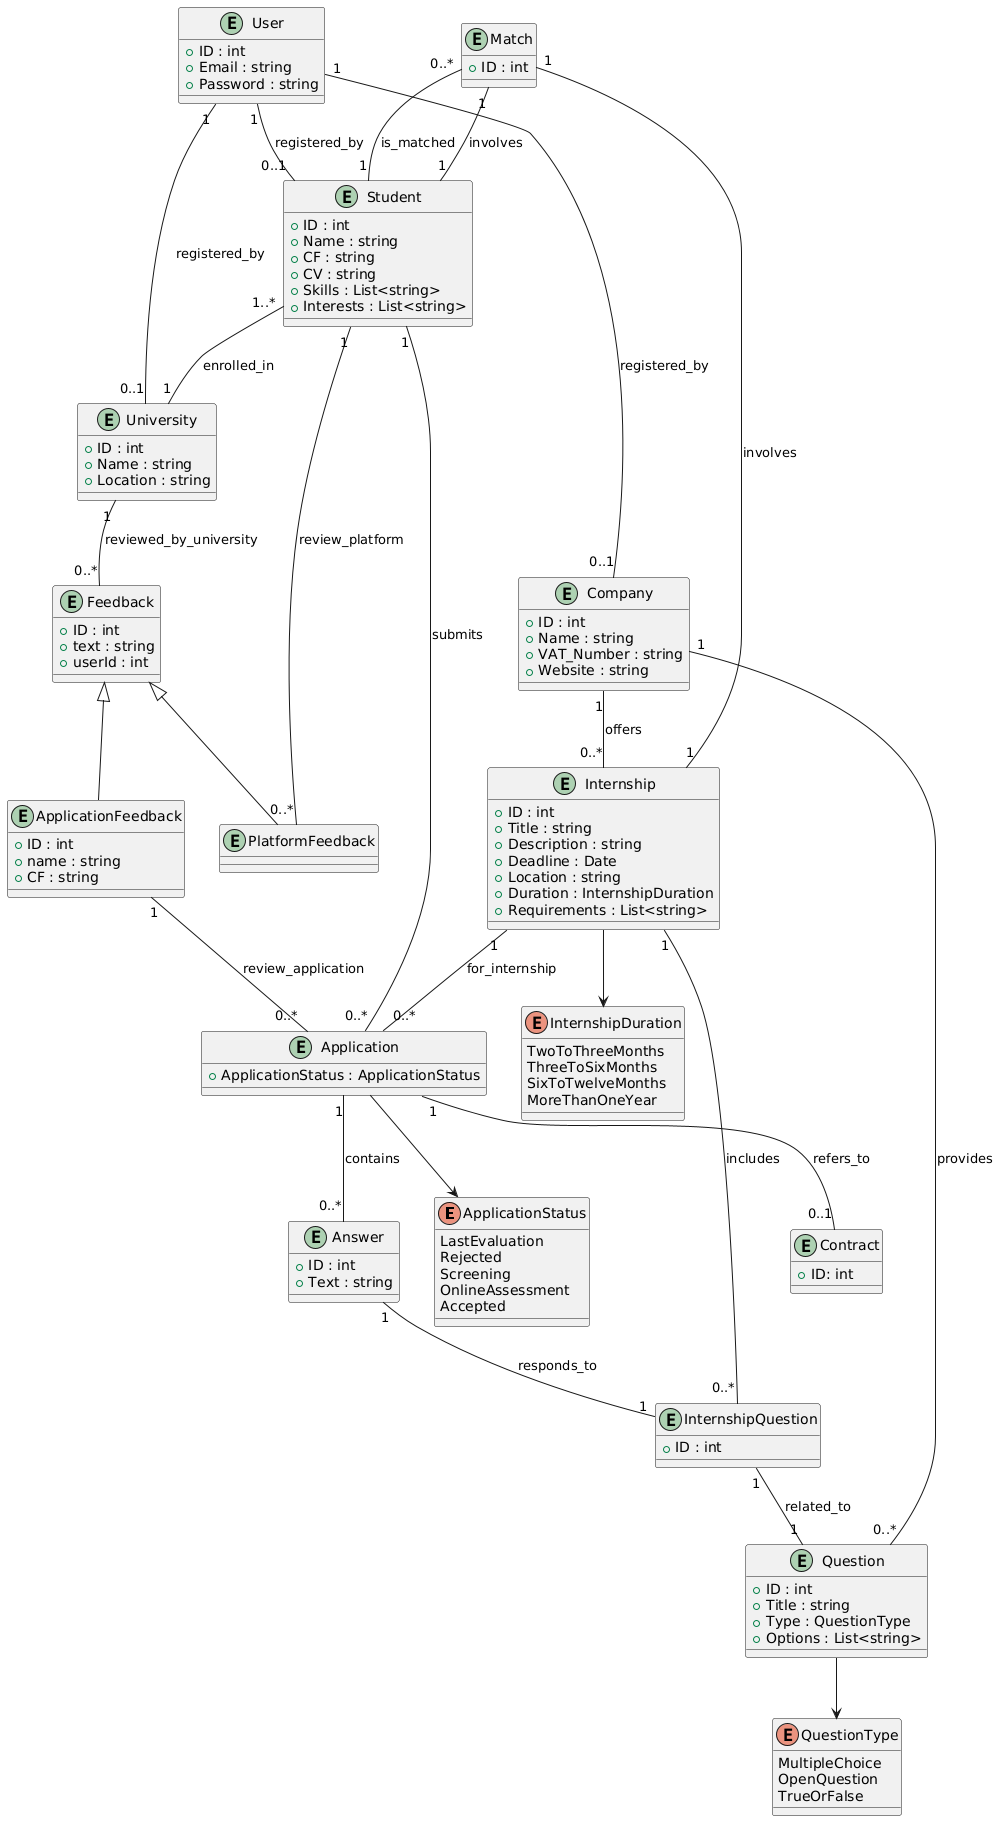
\includegraphics[scale=0.23]{Images/ImagesRASD/domainFinal.png}
    \caption{Class diagram}
\end{figure}

\newpage
\subsection{Scenarios and state diagrams}
The following scenarios illustrate interactions between students, companies, and the S\&C platform.
In order to explain the behavior of some scenarios, we decide to adopt the use of BPMN instead of UML state diagrams, because better describes the exchange of information and messages between the actors (Look for it in the references).

\begin{itemize}
    \item \textbf{Scenario 1: Student registers and uploads CV.}  \\
    Maria, a third-year university student, is looking for internship opportunities to gain practical experience. She discovers the S\&C platform, which connects students with relevant internships. To get started, she navigates to the registration page of the S\&C platform. Maria provides her personal information, including her name, email, university, and sets up a secure password. The platform verifies her email through a confirmation link sent to her inbox. After verifying, Maria is successfully registered and directed to the homepage. By going into her profile section, she completes her profile by specifying her skills and interests, and uploads her CV to showcase her academic background, work experience, and skills. The system securely stores this information and uses it to generate internship recommendations tailored to Maria’s profile. She is informed that she can update her profile over time.

    \begin{figure}[!ht]
    \centering
    \includegraphics[scale=0.30]{Images/ImagesRASD/scenario_1.png}
    \caption{BPMN diagram scenario 1}
    \end{figure}

    \item \textbf{Scenario 2: Company registers.} \\
    CodeWorks, a tech company specializing in front-end development, decides to utilize the S\&C platform to find potential interns. The HR manager at CodeWorks begins by registering the company on the platform. They navigate to the company registration page, where they provide essential details such as the company name, VAT number, location, and a contact email, setting up a password for secure access. After submitting the information, a verification email is sent to the contact email provided. The HR manager completes the verification process by clicking the link, activating the company account on the platform.

    \item \textbf{Scenario 3: Company posts a new internship.} \\
    After creating a profile, CodeWorks is ready to post an internship position. The HR manager logs into the S\&C platform and selects the option to post a new internship. They complete fields for the job title, required skills, internship duration, and inside the description section they can define benefits, such as mentorship and training opportunities. Before submitting, the company must define the questions that will be asked to students in the online assessment phase. After submitting the internship details, the listing becomes visible to students.

    \item \textbf{Scenario 4: Student receives internship recommendations.}  \\
    After setting up her profile, Maria begins exploring opportunities. Based on her profile, the S\&C platform’s recommendation engine suggests internships that align with her background. She receives a curated list of potential matches, including details like the position title, required skills, and company information. As Maria browses, she finds an internship at CodeWorks and decides to apply, with the platform offering further details on the job role expectations and deadlines.

    \item \textbf{Scenario 5: Company reviews applications and selects candidates for interviews.} \\
    CodeWorks reviews submissions for the internship. The HR team logs in to the S\&C platform and accesses a list of applicants, including Maria, with CVs and profile details. After review, CodeWorks shortlists Maria and other candidates for the online assessment. The S\&C platform updates Maria's application status to "Online Assessment," allowing her to independently complete the assessment questions on the platform provided by the company.

    \begin{figure}[!ht]
    \centering
    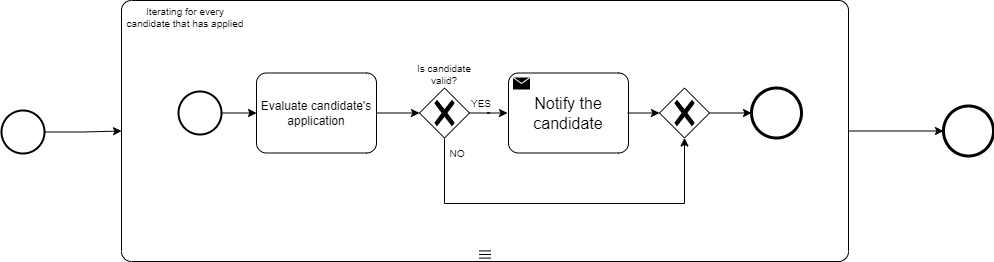
\includegraphics[scale=0.30]{Images/ImagesRASD/scenario_5.png}
    \caption{BPMN diagram scenario 5}
    \end{figure}

    \item \textbf{Scenario 6: The student completes the online assessment, and the company reviews the responses.} \\
    Since Maria was accepted by the company, she now has access to the internship page where she can complete the online assessment by answering the questions prepared by the company. Once completed, she can submit it. After Maria submits her assessment, the company can review it and decide whether to accept her for the internship or exclude her via the application page.

    \item \textbf{Scenario 7: University monitors student internship progress.} \\
    Maria’s university requires students to complete an internship and uses the S\&C platform to monitor student progress. Once Maria secures the internship at CodeWorks, her university’s coordinator views her status, including the start date, role, and completion date. A dashboard allows the coordinator to track Maria’s feedback and address any concerns. If Maria or CodeWorks reports issues, the coordinator is notified, enabling them to assist in resolving challenges like scheduling conflicts or misaligned expectations.

    \item \textbf{Scenario 8: Student Provides Internship Feedback and Receives Evaluation from the Company.}  \\
    After completing her internship at CodeWorks, Maria can provide feedback on her experience by filling out a form and rating her overall satisfaction. Her feedback is anonymized and shared with CodeWorks to support future improvements.
    Similarly, CodeWorks provides feedback by rating Maria with stars and adding comments about her performance. This feedback is visible to companies during her future applications. Students, in turn, can view anonymized comments about the company before deciding to apply.
    \end{itemize}

\newpage

\section{Product Functions}

The Students\&Companies (S\&C) platform serves as an intermediary between students seeking internship opportunities and companies offering them. The primary goal of the platform is to facilitate a streamlined and efficient matchmaking process, providing both students and companies with a robust set of functionalities tailored to their unique needs. Below, the most important requirements of the system are outlined, focusing on core functions that enable users to interact, apply, and manage internships effectively.

\subsection{G1: Students can search for internships that match their skills and career goals.}
\begin{itemize}
    \item R5: Profile editing — The S\&C shall allow students to edit profiles and upload CV.
    \item R6: Skills and interests — The S\&C shall allow students to edit personal details, skills, and interests in their profiles.
    \item R8: Internship search with filters — The S\&C shall provide students with an internship search tool that includes filtering options for location, field of study, and publication date.
\end{itemize}

\subsection{G2: Companies can advertise internships and engage suitable candidates.}
\begin{itemize}
    \item R15: Internship postings — The S\&C shall allow companies to create internship postings, specifying job roles and required skills.
    \item R16: Edit postings — The S\&C shall allow companies to edit existing internship postings after creation.
    \item R17: Dashboard for applications — The S\&C shall allow companies to have a dashboard to review candidate applications and filter profiles.
\end{itemize}

\subsection{G3: The platform can recommend relevant internships to students.}
\begin{itemize}
    \item R5: Profile editing — The S\&C shall allow students to edit profiles and upload CV.
    \item R6: Skills and interests — The S\&C shall allow students to edit personal details, skills, and interests in their profiles.
    \item R9: Tailored recommendations — The S\&C shall allow students to get tailored internship suggestions based on their interests.
    \item R10: Improve recommendation engine — The S\&C shall allow the recommendation engine to improve over time based on feedback from students and companies.
    \item R28: Skill improvement suggestions — The S\&C shall allow suggestions to students on what skills to achieve based on their interests.
\end{itemize}

\subsection{G4: The platform can recommend potential candidates to companies.}
\begin{itemize}
    \item R15: Internship postings — The S\&C shall allow companies to create internship postings, specifying job roles and required skills.
    \item R17: Dashboard for applications — The S\&C shall allow companies to have a dashboard to review candidate applications and filter profiles.
    \item R19: Candidate recommendation feed — The S\&C shall allow companies to have a recommendation feed for candidates based on internship requirements.
    \item R20: Potential candidates — The S\&C shall allow companies access to a "Potential Candidates" feature to view potential matches based on student profiles.
\end{itemize}

\subsection{G5: Companies can manage the selection process through an interview management system.}
\begin{itemize}
    \item R13: View applications — The S\&C shall allow companies to view submitted applications.
    \item R14: Accept or reject candidates — The S\&C shall allow companies to accept or reject candidates directly from the submitted applications.
    \item R17: Dashboard for applications — The S\&C shall allow companies to have a dashboard to review candidate applications and filter profiles.
    \item R18: Application tracking — The S\&C shall allow companies access to a comprehensive page to track applications status.
\end{itemize}

\subsection{G6: Companies can evaluate candidates.}
\begin{itemize}
    \item R13: View applications — The S\&C shall allow companies to view submitted applications.
    \item R14: Accept or reject candidates — The S\&C shall allow companies to accept or reject candidates directly from the submitted applications.
    \item R22: Candidate evaluation — The S\&C shall allow companies to view feedback provided for candidates from previous internships.
\end{itemize}

\subsection{G7: Students and companies can provide feedback to continuously improve the matchmaking process.}
\begin{itemize}
    \item R21: Feedback system — The S\&C shall allow both students and companies to provide feedback, covering overall satisfaction.
    \item R22: Candidate evaluation — The S\&C shall allow companies to view feedback provided for candidates from previous internships.
    \item R23: Company evaluation — The S\&C shall allow students to view feedback provided for companies from previous interns.
    \item R25: Reporting feature — The S\&C shall allow a reporting feature for users to report inappropriate or irrelevant internship environments, ensuring a safe and professional place.
\end{itemize}

\subsection{G8: Universities can track and assess the ongoing progress of internships.}
\begin{itemize}
    \item R24: Feedback monitoring — The S\&C shall allow universities to monitor feedback scores to ensure professional standards are met during internships.
    \item R26: University feedback — The S\&C shall allow universities to write feedback on the platform to suggest improvements.
    \item R27: Direct feedback — The S\&C shall allow universities to write feedback directly to students and companies.
\end{itemize}

\subsection{G9: The platform can provide suggestions to improve CVs.}
\begin{itemize}
    \item R5: Profile editing — The S\&C shall allow students to edit profiles and upload CV.
    \item R6: Skills and interests — The S\&C shall allow students to edit personal details, skills, and interests in their profiles.
    \item R28: Skill improvement suggestions — The S\&C shall allow suggestions to students on what skills to achieve based on their interests.
\end{itemize}

\subsection{G10: The platform can provide suggestions to companies to improve internship description.}
\begin{itemize}
    \item R15: Internship postings — The S\&C shall allow companies to create internship postings, specifying job roles and required skills.
    \item R16: Edit postings — The S\&C shall allow companies to edit existing internship postings after creation.
    \item R29: Description suggestion - The S\&C shall allow the platform to provide suggestions to companies for improving the quality and clarity of their internship descriptions.
\end{itemize}

\section{User Characteristics}

The Students\&Companies (S\&C) platform is designed to cater to three primary types of users: students, companies, and universities. Each user group has unique needs and characteristics, which the platform addresses to ensure a user-friendly and effective experience. Understanding these user characteristics is essential for aligning the platform’s functionalities with user expectations and optimizing their interactions.

\subsection{Students}
Students are the primary user group for the S\&C platform. Generally, they are undergraduate or graduate students from diverse academic backgrounds, including engineering, business, arts, and sciences. Students are often in search of practical experience, skill development, and improved employability, making internships highly valuable for their career growth. \\ \\
The platform supports students by providing access to internship opportunities that match their specific skills, academic background, and career aspirations. With a simplified application process, students can easily apply for internships and submit their CVs directly through the platform, making the process efficient and accessible. To enhance the likelihood of securing a position, students receive notifications about recommended internships aligned with their profile, ensuring they don’t miss out on opportunities. Additionally, students can track the status of their applications, allowing them to stay informed about each step of the process. To further support career development, the S\&C platform offers students guidance on improving their CVs and profiles, enhancing their chances of selection for internships.

\subsection{Companies}
Companies on the S\&C platform range from small startups to large enterprises across various industries, each seeking talented interns who can support their teams, bring fresh perspectives, and contribute to ongoing projects. \\ \\
For companies, the S\&C platform offers a straightforward registration process and an intuitive interface to post internships, allowing them to quickly reach a large pool of qualified students. Companies benefit from easy access to student profiles and CVs, enabling them to identify candidates with the skills and experiences that best fit their requirements. The platform also provides tools to manage applications efficiently, from the review stage through to collecting questions from the students. Companies can leave feedback to improve future offerings and to enhance the platform’s recommendation algorithms.

\subsection{Universities}
Universities, particularly those involved in career services or specific academic departments, use the platform to oversee their students’ internship experiences and ensure they align with the enstablished requirements. This group may include career service coordinators, faculty advisors, and program managers who play an active role in supporting students during their internships.\\ \\
For universities, the S\&C platform includes a monitoring dashboard that allows administrators to track students’ internship statuses, review both student and company feedback, and provide support when necessary. This feature is essential for maintaining an overview of students’ progress and ensuring that internships meet academic standards. Additionally, administrators can mediate any complaints or issues that arise between students and companies, facilitating resolution and safeguarding the quality of the internship experience.
\\ \\

\section{Assumptions, Dependencies, and Constraints}
\begin{itemize}
    \item \textbf{Internet Availability}: The platform assumes users have access to a stable internet connection to interact with the web-based interface.
    \item \textbf{Data Privacy}: The platform must comply with GDPR regulations, ensuring that all personal data from students and companies is handled securely and transparently.
    \item \textbf{Scalability}: The system must be able to scale to accommodate multiple universities and thousands of users simultaneously.
    \item \textbf{Cross-browser Compatibility}: The platform should work on all major browsers (e.g., Chrome, Firefox, Safari) and on both desktop and mobile devices.
\end{itemize}

\section{Domain Assumptions}
\begin{longtable}{|p{1cm}|p{4cm}|}
\hline
\textbf{ID} & \textbf{Assumption} \\
\hline
\textbf{DA1} & Students have varied skills and interests \\
\hline
\textbf{DA2} & Companies have specific internship requirements \\
\hline
\textbf{DA3} & The students need to provide a valid email address \\
\hline
\textbf{DA4} & The companies need to provide a valid email \\
\hline
\textbf{DA5} & The universities need to have a valid email \\
\hline
\textbf{DA6} & Both parties (students and companies) need to have a connection and a device to connect to the platform \\
\hline
\textbf{DA7} & The student and the university successfully register as a student and university, respectively. \\
\hline
\textbf{DA8} & Students are enrolled in the university they selected. \\
\hline
\textbf{DA9} & The company account accurately corresponds to the respective company. \\
\hline
\end{longtable}
\newpage